\newpage
\section{Complete mechanism and components description}

In this section it will be explained how the overall final mechanism and each of its components work, including photos from different views for the whole mechanism and the gripper, and a single photo for each component in detail. Dimensions will be indicated as well.

\subsection{Mechanism overview}
From the different views shown in the next page, it can be noticed that the half-shaft end joint is positioned in a perfectly cut slot in the transport tray it is laid on. All the grasping process, whenever the object reaches the destination where it must be lifted, is done by the modified \texttt{Jodell} gripper, which will descend precisely on the shown position to guarantee a solid grip. When the descending phase has ended, it will envelop the non-threaded part of the cylinder, while a buffer positioned on the threaded part (very close to its end) efficiently exerts a force that counters the momentum generated by gravity. The envelop process, carried out by the claws, will only start when the buffer touches the shaft, so that the part will be lifted horizontally. In fact, without it it can be easily assessed that the part would incline in the direction of its centre of mass. Then the gripper will bring the shaft wherever it needs to be in a stabilized way. Every part of the modified gripper that will touch the cylinder is coated with a small rubber layer, as said before. \texttt{Figure 3} was obtained without the tray to give a clearer view of the gripper positioned near to the half-shaft, ready for grabbing. 
\vspace{0.5pt}

\begin{figure}[H]
    \centering
    \begin{minipage}{0.45\textwidth}
        \centering
        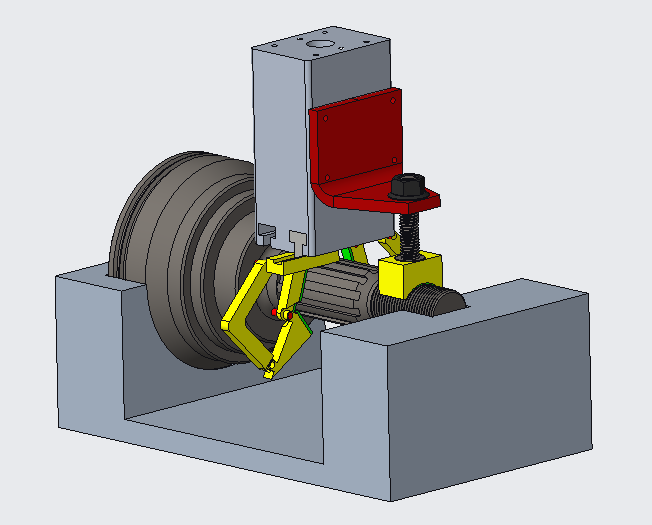
\includegraphics[width=\textwidth]{Immagini/mechanism.png}
        \caption{Mechanism}
    \end{minipage}
    \hfill
    \begin{minipage}{0.45\textwidth}
        \centering
        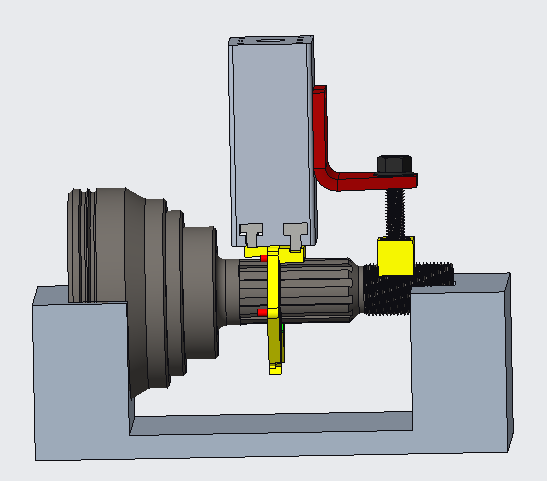
\includegraphics[width=\textwidth]{Immagini/mechanism side.png}
        \caption{Mechanism side view}
    \end{minipage}
\end{figure}

\begin{figure}[H]
    \centering
    \begin{minipage}{0.45\textwidth}
        \centering
        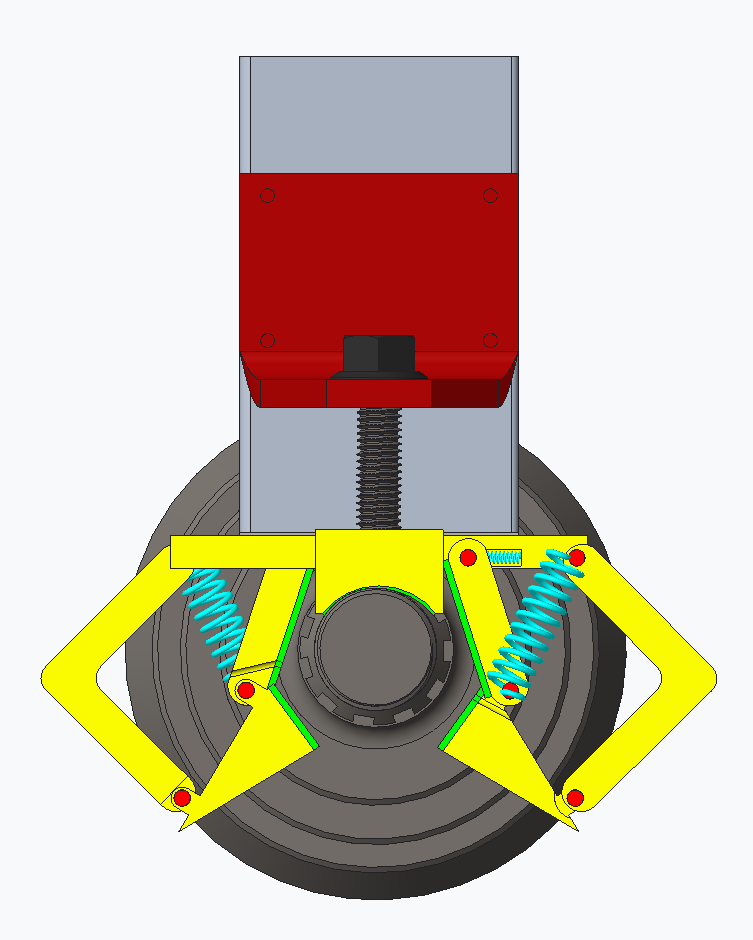
\includegraphics[width=0.7\textwidth]{Immagini/mechanism front.png}
        \caption{Mechanism front view}
    \end{minipage}
    \hfill
    \begin{minipage}{0.45\textwidth}
        \centering
        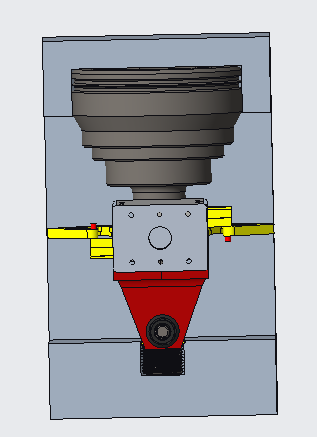
\includegraphics[width=0.7\textwidth]{Immagini/mechanism up.png}
        \caption{Mechanism upper view}
    \end{minipage}
\end{figure}


\subsection{Modified \texttt{Jodell} gripper analysis}
Here, the principal design decision of the \texttt{Jodell} gripper that brought to this definitive design was conditioned by the need to grasp the same object but with different possible section dimensions considering the market availability. The result of a brief research on these dimensions was a range from $25\text{ mm}$ to $35\text{ mm}$, consisting of the $90\%$ of the half-shaft end joints in the automotive market. The internal gum layers are made of high density expanded neoprene and low density expanded polyethylene. As can be seen from \texttt{Figure 8}, the two quadrilateral claws are mounted on two sliders which are positioned in two specific slots. These are put in two grooves created on the base body of the gripper. The functioning process provides that the sliders will bring the proximal links close to the cylinder until they touch it. Then, because of the upper revolute joints and of the way the claws were designed, they will start to envelop the lower part of the cylinder with the triangular pieces. The movement is constrained with springs to resist the gravitational force pushing down the half-shaft end joint during the lift process. 

\begin{figure}[H]
    \centering
    \begin{minipage}{0.49\textwidth}
        \centering
        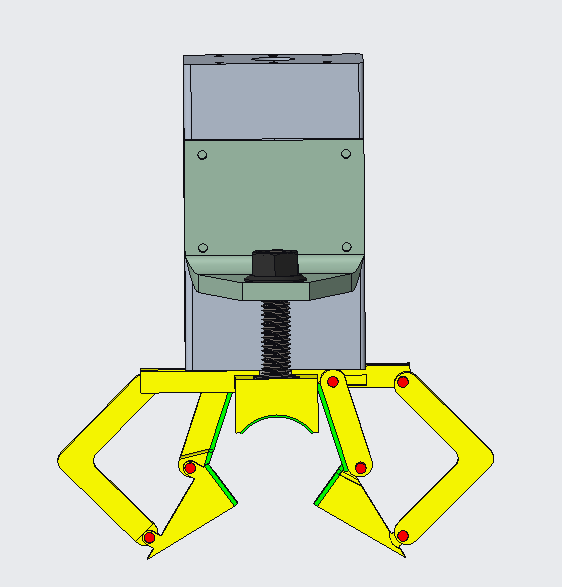
\includegraphics[width=\textwidth]{Immagini/Jodell gripper/jodell fronte.png}
        \caption{\texttt{Jodell} gripper front view}
    \end{minipage}
    \hfill
    \begin{minipage}{0.45\textwidth}
        \centering
        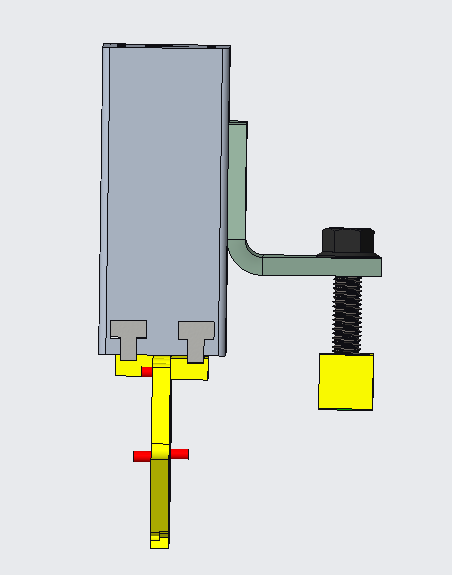
\includegraphics[width=\textwidth]{Immagini/Jodell gripper/jodell side.png}
        \caption{\texttt{Jodell} gripper side view}
    \end{minipage}
\end{figure}

\begin{figure}[H]
    \centering
    \begin{minipage}{0.48\textwidth}
        \centering
        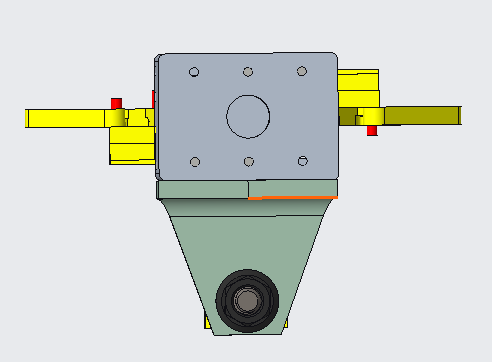
\includegraphics[width=\textwidth]{Immagini/Jodell gripper/jodell alto.png}
        \caption{\texttt{Jodell} gripper upper view}
    \end{minipage}
    \hfill
    \begin{minipage}{0.45\textwidth}
        \centering
        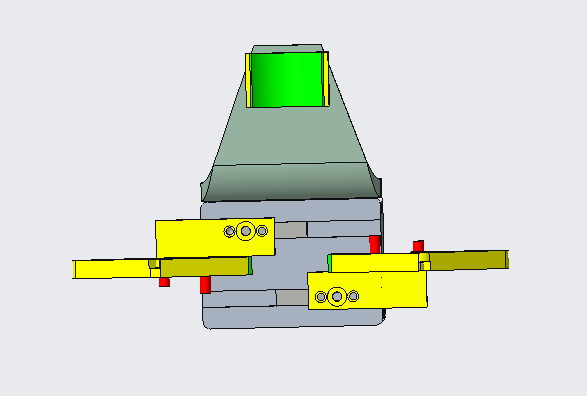
\includegraphics[width=\textwidth]{Immagini/Jodell gripper/jodell sotto.png}
        \caption{\texttt{Jodell} gripper underneath view}
    \end{minipage}
\end{figure}

\subsection{Parts analysis}

\subsubsection{Base of the claw and slider}

Here the main base of the claws can be seen in \texttt{Figure 9}: its upper groove hosts the bottom surface of the slider mounted on the main body of the \texttt{Jodell} gripper (\texttt{Figure 10}). The contact only interests half of both, for functioning purposes, as shown in \texttt{Figure 11}. Then, when the gripper will come in contact with the shaft through the buffer, the \texttt{Jodell} gripper sliders will move on their resting position to the inside until the claws touch the cylinder they are supposed to grasp. The red parts are two revolute joints firstly used to connect the claw to its base, secondly to make it rotate after touching the cylinder with the proximal links of the mechanism. The cubic blue part inside the lateral groove, which houses the shorter revolute joint, is attached to one of the two sprigs per claw. It is useful to compress the spring attached to it when the proximal link has already come in contact with the cylinder. Then, as will be explained later, the slider continues to move along its direction compressing the spring, which allows to keep the proximal link in contact with the cylinder and actuating the rest of the movement of the claws to complete the grasping process.

\begin{figure}[H]
    \centering
    \begin{minipage}{0.30\textwidth}
        \centering
        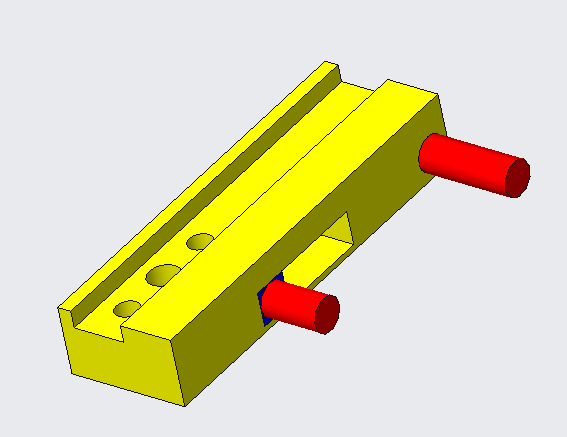
\includegraphics[width=1\textwidth]{Immagini/Jodell gripper/Claw/base claw 2.png}
        \caption{Base of the claw}
    \end{minipage}
    \hfill
    \begin{minipage}{0.30\textwidth}
        \centering
        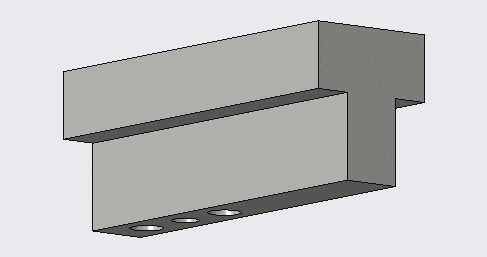
\includegraphics[width=1\textwidth]{Immagini/Jodell gripper/Claw/gripperconnector.png}
        \caption{Slider}
    \end{minipage}
    \hfill
    \centering
    \begin{minipage}{0.30\textwidth}
    	\centering
    	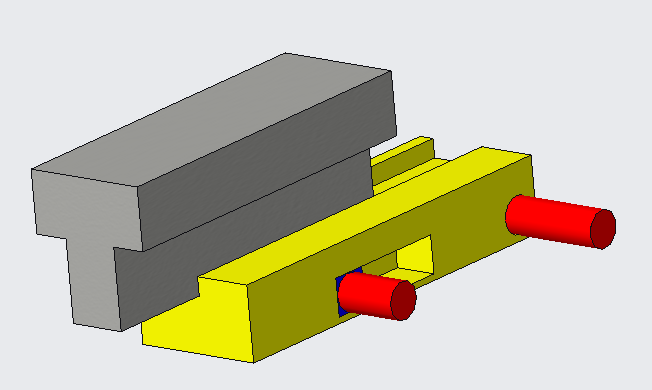
\includegraphics[width=1\textwidth]{Immagini/Jodell gripper/Claw/slider + base.png}
    	\caption{Claw base mounted on the slider}
    \end{minipage}
    
\end{figure}

The sliding base has a dimension of $35\text{ mm}$ when at rest, defining a trapezoidal mechanism, while it has a dimension of $25\text{ mm}$ at maximum compression (when the cylinder is touched only with a sliding movement). The useful stroke of the slider corresponds to $10$--$12\text{ mm}$.

\vspace{0.5cm}
\subsubsection{Proximal link, distal link and triangular hugger}

\begin{figure}[H]
    \begin{minipage}{0.45\textwidth}
        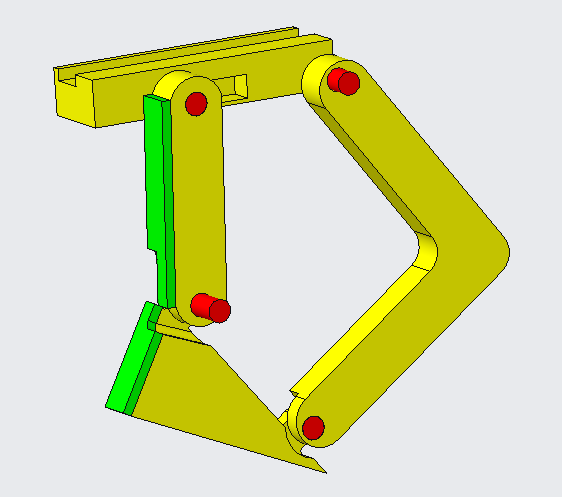
\includegraphics[width=\textwidth]{Immagini/Jodell gripper/Claw/claw3.png}
        \caption{Claw mechanism}
    \end{minipage}
    \hfill
    \begin{minipage}{0.45\textwidth}
    Here is shown the complete mechanism of the claw, whose task is to basically hug the shaft cylindrical part to securely lift it (cooperating with the buffer). Every part that composes it can be clearly seen: the base of the claw housing the slider of the \texttt{Jodell}, the shorter proximal link (the first to touch the cylinder), the longer L-shaped distal link and the triangular hugger, which is fundamental to correctly perform the grasp.
    \end{minipage}
\end{figure}

\begin{figure}[H]
    \begin{minipage}{0.35\textwidth}
        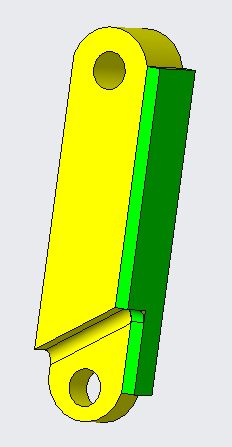
\includegraphics[width=0.7\textwidth]{Immagini/Jodell gripper/Claw/prossimale.png}
        \centering
        \caption{Proximal link}
    \end{minipage}
    \hfill
    \begin{minipage}{0.55\textwidth}
    The shorter, proximal link (\texttt{Figure 13}) is the first to come in contact with the shaft cylinder. The touch happens in two phases: the first only after a sliding movement of the slider mounted on the main body of the \texttt{Jodell}, until the proximal link touches the cylindrical part of the shaft. The second phase begins when, having the link already in contact, it is maintained like that by the spring in the base of the claw.
    The contact surface is covered with a thin layer of elastic rubber-like material (as said in the description of the \texttt{Jodell} modified manipulator at page $2$). The direct distance between the holes (that will host the revolute joints) measures $45\text{ mm}$.
    \end{minipage}
\end{figure}

\begin{figure}[H]
    \begin{minipage}{0.4\textwidth}
        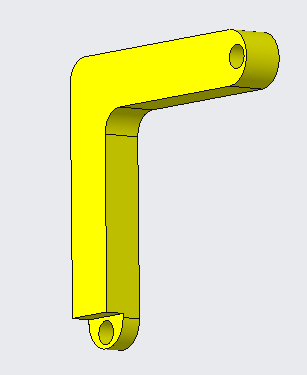
\includegraphics[width=0.8\textwidth]{Immagini/Jodell gripper/Claw/distalee.png}
        \centering
        \caption{Distal link}
    \end{minipage}
    \hfill
    \begin{minipage}{0.55\textwidth}
    As the claw keeps sliding, the rest of the mechanism performs a rotation movement to envelop the bottom surface of the cylinder itself. The main protagonists are the distal link (\texttt{Figure 14}) and the triangular hugger (\texttt{Figure 15}). Here, the distal link allows the hugger to perform the required rotation movement together with the movement of each other part. It as a L-shaped (or elbow-shaped) structure where the tip of it needs to stick out of $20\text{ mm}$ from the line connecting the centers of the two holes, to create the cradle that accommodates a diameter dimension of $35\text{ mm}$ without bumps. The direct distance between the holes (that will host the revolute joints) measures $45\text{ mm}$.
    \end{minipage}
\end{figure}

\begin{figure}[H]
    \begin{minipage}{0.40\textwidth}
        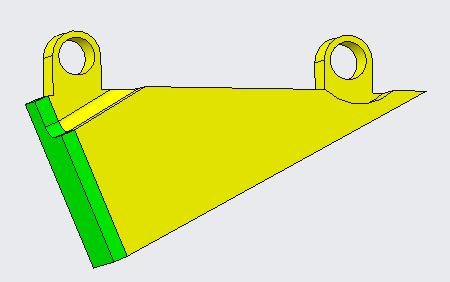
\includegraphics[width=\textwidth]{Immagini/Jodell gripper/Claw/triangolo.png}
        \centering
        \caption{Triangular hugger}
    \end{minipage}
    \hfill
    \begin{minipage}{0.55\textwidth}
    The triangular hugger here is the last component of the claw which makes the mechanism a closed one, the shorter side is the one which comes in contact with the surface of the cylinder together with the proximal link, so it is coated with the same rubber layer. The distance between the holes measures $25\text{ mm}$. It can be seen from the image that two grooves were performed on the surface near the holes. That is made to avoid collisions with the two links above it during the rotation.
    \end{minipage}
\end{figure}

\subsubsection{Springs utilization}
\label{sec:springs}

\begin{figure}[H]
    \centering
    \begin{minipage}{0.45\textwidth}
        \centering
        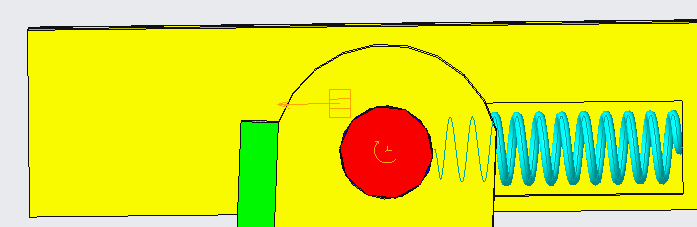
\includegraphics[width=\textwidth]{Immagini/Jodell gripper/Claw/molle1.png}
        \caption{First spring in the base of the claw}
    \end{minipage}
    \hfill
    \begin{minipage}{0.50\textwidth}
        \centering
        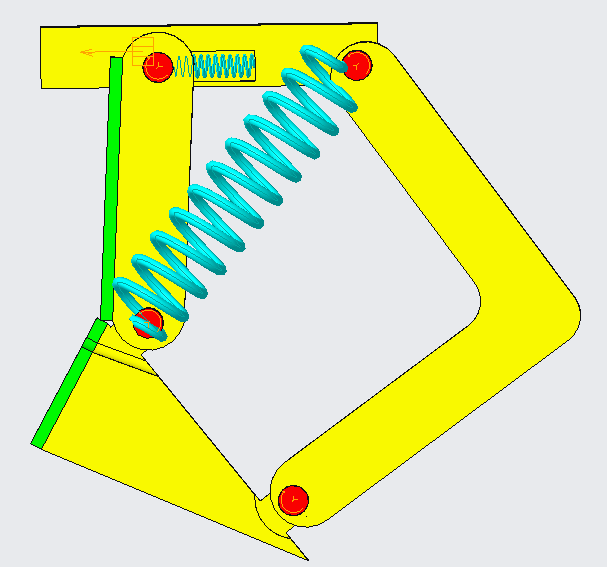
\includegraphics[width=\textwidth]{Immagini/Jodell gripper/Claw/molla2.png}
        \caption{Second spring between the hugger and the distal link}
    \end{minipage}
\end{figure}

All the springs, shown only via the \texttt{Creo Mechanism} window, serve two purposes:
\begin{itemize}
	\item \texttt{\textbf{When not in contact:}} to keep the claws in a constant stable position, to ensure the correct initialization of the robot actions. This position is kept stable during the approaching phase of the claw to the cylinder, in order to generate the first contact between it and the proximal link. 
	\item \texttt{\textbf{When in contact:}} to grant the adaptability of the mechanism and the dynamic of the movement. During this phase, the action of the springs allows the links to rotate in such way to correctly envelop the cylinder, keeping the grip stabilized. While in the first phase only a translational movement interested the links of the claw, during the second phase rotational movements are the main ones.

\end{itemize}

\vspace{1cm}
\subsubsection{Mechanical buffer}

The second part of the modified gripper consists of the stabilization system which is formed by the mechanical buffer (\texttt{Figure 18}). It helps to stabilize the positioning of the shaft when lifted by maintaining it in a horizontal position during all the movement. More precisely, this happens by only touching the threaded part of the cylindrical portion of the half-shaft with its rubber end, which will generate a resisting force that will counter the momentum generated by the gravity force. In fact, the physical constitution of the half-shaft clearly shows that the centre of mass is placed near the part with the biggest section. This surely makes the piece tilt when trying to lift it only with the claw part of the gripper, because of the gravity force. So it is needed a stabilization system like it was designed.
Mechanically, it is composed by a sheet metal mounted on the side of the \texttt{Jodell} main body (\texttt{Figure 22}), a M8 nut with flange and a thread pitch of $1{,}25$ (\texttt{Figure 20}), a screw of the type DIN 912 M8X30F A2 (same thread pitch of the nut) (\texttt{Figure 19}) and a rubber extremity (\texttt{Figure 21}). The sheet metal represents the fixed support on which the rest of the buffer is built. In fact, a hole of diameter $7{,}5\text{ mm}$ was created at the extremity of the horizontal part of the sheet metal. The screw has a diameter of $8\text{ mm}$ so the slightly restricted section of the hole allows a solid fit. The screwing distance can be regulated basing on the correct positioning of the gripping part, considering that the maximum length of the screwable part is of $30\text{ mm}$ measured from the screw head. To better stabilize the screw, a nut with a flange ($8\text{ mm}$ in diameter) is put on top of the hole laying on the sheet metal in that position. Then, the rubber swab has a hole carved in to house the head of the screw. The diameter of the head is $12{,}4\text{ mm}$. 


\begin{figure}[H]
	\vspace{2cm}
    \centering
    \begin{minipage}{0.30\textwidth}
        \centering
        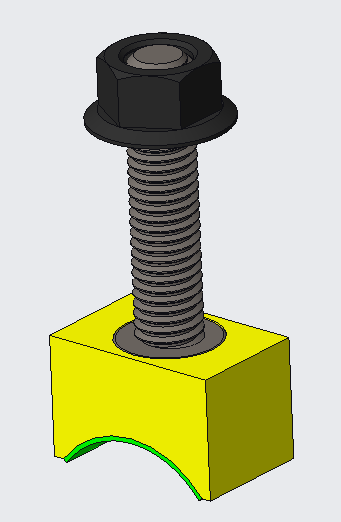
\includegraphics[width=\textwidth]{Immagini/tampone/tampone full.png}
        \caption{Mechanical buffer}
    \end{minipage}
    \hspace{3cm}
    \begin{minipage}{0.25\textwidth}
        \centering
        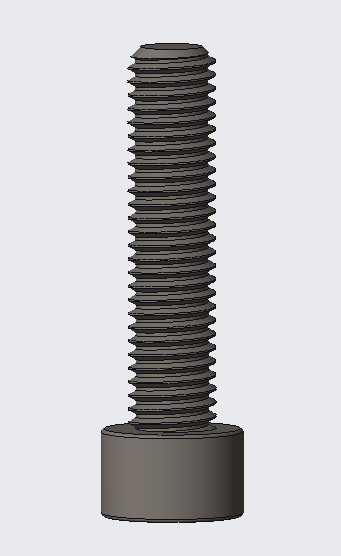
\includegraphics[width=\textwidth]{Immagini/tampone/vite.png}
        \caption{DIN 912 M8X30F A2 screw}
    \end{minipage}
\end{figure}

\begin{figure}[H]
    \centering
    \begin{minipage}{0.30\textwidth}
        \centering
        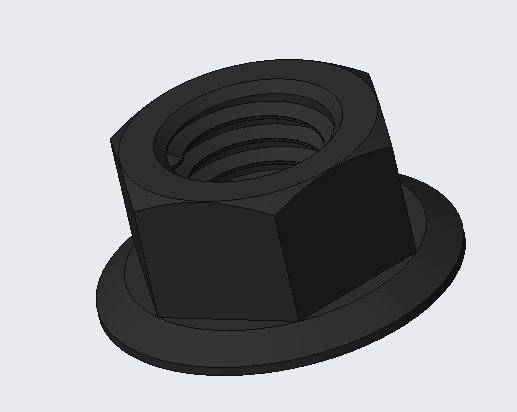
\includegraphics[width=\textwidth]{Immagini/tampone/dado.png}
        \caption{M8x1,25 nut with flange}
    \end{minipage}
    \hspace{2cm}
    \begin{minipage}{0.30\textwidth}
        \centering
        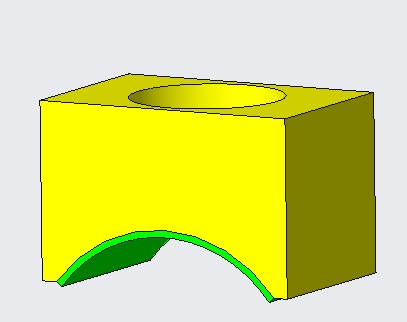
\includegraphics[width=\textwidth]{Immagini/tampone/tampone.png}
        \caption{Rubber swab}
    \end{minipage}
\end{figure}

\begin{figure}[H]
    \centering
    \begin{minipage}{0.35\textwidth}
        \centering
        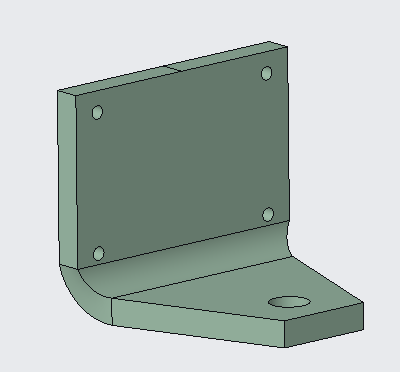
\includegraphics[width=\textwidth]{Immagini/tampone/braccio.png}
        \caption{Sheet metal}
    \end{minipage}
    \hspace{2cm}
    \begin{minipage}{0.35\textwidth}
        \centering
        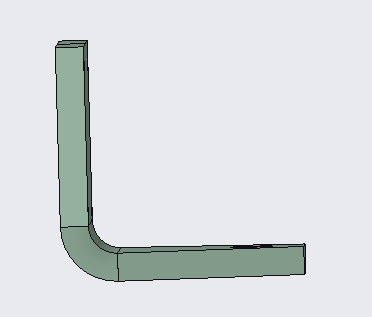
\includegraphics[width=\textwidth]{Immagini/tampone/braccio side.png}
        \caption{Sheet metal side view}
    \end{minipage}
\end{figure}

\vspace{4cm}
\subsubsection{Kinematic closing sequence}
The claw mechanism described above can be summarized as a serial kinematic chain composed of one prismatic pair and three revolute pairs (P--R--R--R): the prismatic pair corresponds to the \texttt{Jodell} slider, while the three revolute pairs connect, in sequence, the claw base to the proximal link, the proximal link to the distal link, and the distal link to the triangular hugger. The closing action unfolds in the following steps:

\begin{enumerate}
    \item \textbf{Linear actuation (P):} the \texttt{Jodell} sliders translate rigidly toward the half-shaft, carrying the claw bases and the buffer support along a purely linear trajectory.
    \item \textbf{Contact and stabilization:} the buffer's rubber end is the first element to reach the shaft, touching the threaded section and generating the counter-moment needed to keep the half-shaft horizontal before any radial grasping force is applied.
    \item \textbf{Passive envelopment (R--R--R):} once the proximal link makes contact with the cylindrical section, the reaction force compresses the base spring (Section~\ref{sec:springs}), which in turn actuates the rotation of the distal link and triangular hugger about their revolute joints, wrapping the claw around the shaft until the grasp is complete.
\end{enumerate}

This sequence highlights that only the first phase is actively driven by the \texttt{Jodell} motor, while the remaining degrees of freedom are closed passively through the spring-loaded linkage, consistently with the under-actuated nature of the mechanism.

\subsubsection{Tray}
The tray is where the half-shaft is placed on. It contains two semi-circular carved parts which have the same sections of the respective ends of the object it must contain. Respectively, the sections measure $90\text{ mm}$ for the head of the shaft slot diameter and $23\text{ mm}$ for the threaded end slot diameter. The lateral vertical sides of the tray extremities are not carved because they must not allow horizontal movements of the shaft during the transport. All of this can be seen in the subsequent images. 

\begin{figure}[H]
    \centering
    \begin{minipage}{0.65\textwidth}
        \centering
        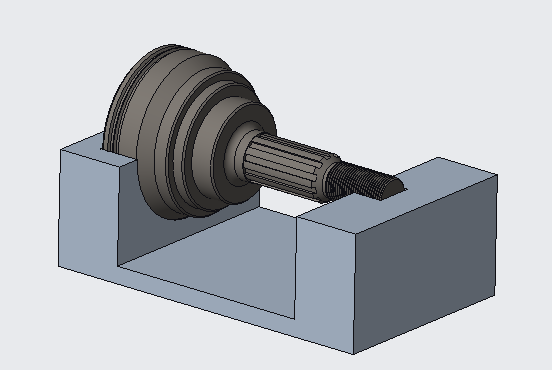
\includegraphics[width=\textwidth]{Immagini/vassoio/vassoio con pezzo.png}
        \caption{Tray containing the half-shaft}
    \end{minipage}
\end{figure}

\begin{figure}[H]
    \centering
    \begin{minipage}{0.65\textwidth}
        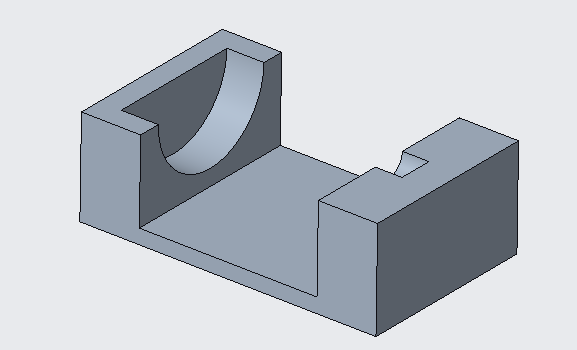
\includegraphics[width=\textwidth]{Immagini/vassoio/vassoio.png}
        \caption{Empty tray}
    \end{minipage}
\end{figure}

\subsection{Parts assembly}

This subsection shows how the components explained in this chapter are assembled to form the final design. This is done by using Creo Parametric's View functionality, more specifically using explode views that allow the components to be temporarily separated without harming the real assembly. For the sake of simplicity and to avoid excessive cluttering, the explode view is shown below both for the singular claw and for the jodell component with the whole claws.

\begin{figure}[H]
	\centering
	\begin{minipage}{0.35\textwidth}
		\centering
		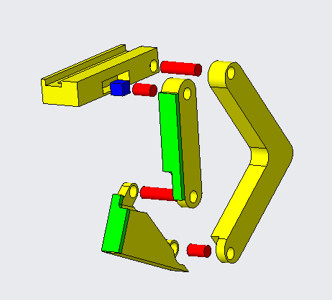
\includegraphics[width=\textwidth]{Immagini/claw_anchorless_espl}
		\caption{Claw exploded view}
	\end{minipage}
	\hspace{2cm}
	\begin{minipage}{0.35\textwidth}
		\centering
		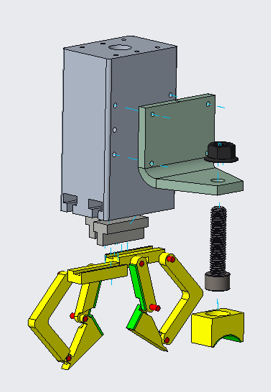
\includegraphics[width=\textwidth]{Immagini/jodell_espl}
		\caption{Jodell assembly exploded view}
	\end{minipage}
\end{figure}

\subsection{Requirement verification}
This section verifies how the final design presented above satisfies the requirements and constraints formally introduced in Section~1.2.

\begin{table}[H]
\centering
\caption{Requirement verification table}
\label{tab:requirement-verification}
\renewcommand{\arraystretch}{1.4}
\begin{tabular}{|p{2.7cm}|p{4.6cm}|p{6.2cm}|}
\hline
\rowcolor{black}
\textcolor{white}{\textbf{Requirement}} &
\textcolor{white}{\textbf{Description}} &
\textcolor{white}{\textbf{How it is satisfied}} \\
\hline
Diameter range & Grasp sections between $25$--$35\text{ mm}$ & The under-actuated quadrilateral claw, combined with the $10$--$12\text{ mm}$ slider stroke, closes on any diameter within this range without manual reconfiguration. \\
\hline
No-touch zones & Avoid splines, ball cage and both threaded sections & The claws contact only the $28\text{ mm}$ non-threaded cylindrical section, while the buffer contacts the $23\text{ mm}$ threaded section exclusively along its axis, never radially. \\
\hline
Surface protection & Prevent wear and slipping on delicate finishes & Every contact point (claws, hugger, buffer tip) is coated with a rubber layer that absorbs clamping force and prevents metal-on-metal contact. \\
\hline
Load stability & Counteract the gravity-induced moment caused by the off-centered mass & The mechanical buffer engages the threaded section before the claws close, generating a counter-moment that keeps the half-shaft horizontal throughout the lift. \\
\hline
Compatibility & Operate using only the \texttt{Jodell} linear sliders & The whole claw kinematics (P--R--R--R chain, Section~3.3.4) is driven by the two existing sliders; no additional actuator was introduced. \\
\hline
\end{tabular}
\end{table}
